\section{Finite Volume Method for the Shallow Water Equations}
In this section we will describe the Finite Volume Method (FVM) for solving nonlinear systems of balance laws, such as the shallow water equations (SWE).
That is, we consider the FVM for nonlinear hyperbolic conservation laws, such as the shallow water equations.
The nonlinear case is obviously more challenging than the linear case, as stability and convergence theory are more difficult.
We are interested in discountinuous solutions, which can capture shock waves and other discontinuities in the solution.
The method described is based on the book by LeVeque~\cite{LeVeque2002}.


In finite volume methods, we discretize the domain into cells or control volumes.
Then we solve the local Riemann problem at the cell interface to obtain the fluxes.
Using the computed fluxes, we update the solution in each cell.
This way, the FVM allows for discountinuous solutions, as we solve the Riemann problem at the cell interfaces.
Therefore it is well suited for hyperbolic conservation laws, such as the shallow water equations.



\subsection{Finite Volume Methods for the 1D SWE}
We begin by considering finite volume methods for the SWE in one space dimension.
In the FVM, we discretize the domain into finite control volumes or cells:
\begin{align*}
    V_i = [x_{i-1/2}, x_{i+1/2}] \times [t_n, t_{n+1}],
\end{align*}
where $\Delta x = x_{i+1/2} - x_{i-1/2}$ is the length of the cell and $\Delta t = t_{n+1} - t_n$ is the time step.
The cell $V_i$ is illustrated in Figure~\ref{fig:control_volume_V_i_n}.
\begin{figure}[H]
    \centering
    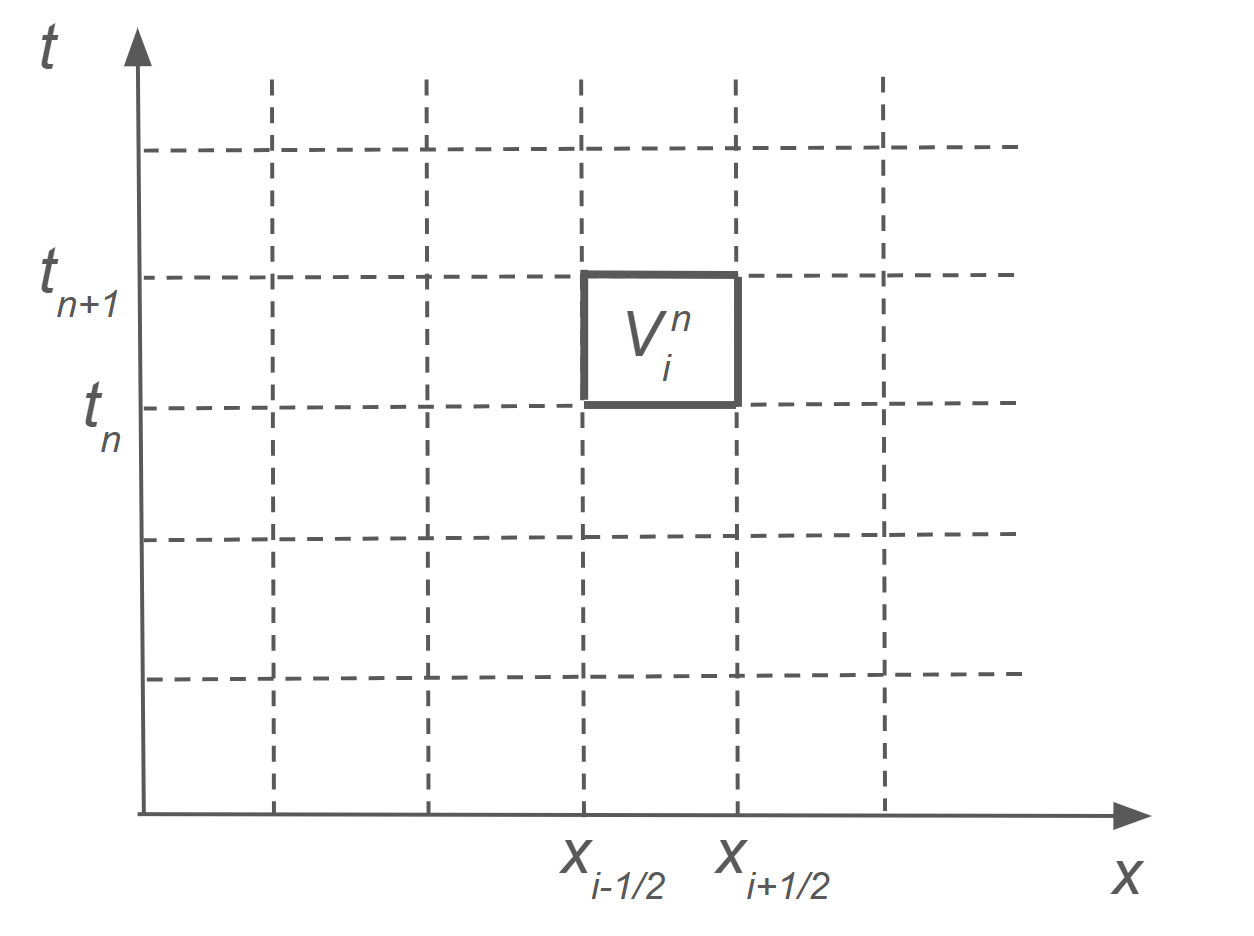
\includegraphics[width=0.4\textwidth]{C:/Users/Matteo/Shallow-Water-Equations/tex/figs/control_volume_V_i_n.png}
    \caption{Illustration of the control volume $V_i^n$ in the $x-t$ plane.}\label{fig:control_volume_V_i_n}
\end{figure}
For now, we will assume a uniform grid for simplicity.
The Finite Volume Formula is derived from the integral form~\eqref{eq:integral_form_1D_final}.
By dividing this by the cell length $\Delta x$, we espress it in terms of the newly defined cells:
\begin{align*}
    \frac{1}{\Delta x} \int_{x_{i-1/2}}^{x_{i+1/2}} \mathbf{U}(x,t_{n+1}) \text{ d}x &= \frac{1}{\Delta x} \int_{x_{i-1/2}}^{x_{i+1/2}} \mathbf{U}(x,t_n) \text{ d}x\\
    & - \frac{\Delta t}{\Delta x} \left[ \frac{1}{\Delta t} \int_{t_n}^{t_{n+1}} \mathbf{F}(\mathbf{U}(x_{i+1/2}, t)) \text{ d}t
    - \frac{1}{\Delta t} \int_{t_n}^{t_{n+1}} \mathbf{F}(\mathbf{U}(x_{i-1/2}, t)) \text{ d}t \right] \\
    &+ \frac{\Delta t}{\Delta x \Delta t} \int_{x_{i-1/2}}^{x_{i+1/2}} \int_{t_n}^{t_{n+1}} \mathbf{S(U)}(x,t) \text{d}x \text{d}t.
\end{align*}
For a finite volume $V_i^n$, averaging the terms over the volume yields the explicit conservative form
\begin{align}\label{eq:explicit_conservative_1D_SWE}
    \mathbf{U}_i^{n+1} = \mathbf{U}_i^n - \frac{\Delta t}{\Delta x} \left( \mathbf{F}_{i+1/2}^n - \mathbf{F}_{i-1/2}^n \right) + \Delta t \mathbf{S}_i.
\end{align}
Here, $\mathbf{U}_i^n$ is the average value over the $i$-th cell at time $t_n$:
\begin{align}
    \mathbf{U}_i^n = \frac{1}{\Delta x} \int_{x_{i-1/2}}^{x_{i+1/2}} \mathbf{U}(x,t_n) \text{ d}x,
\end{align}
also known as the cell average.
The flux $\mathbf{F}_{i-1/2}^n$ is the average flux across the line $x = x_{i-1/2}$ at time $t_n$:
\begin{align*}
    \mathbf{F}_{i-1/2}^n = \frac{1}{\Delta t} \int_{t_n}^{t_{n+1}} \mathbf{F}(\mathbf{U}(x_{i-1/2},t)) \text{ d}t,
\end{align*}
while the source term $\mathbf{S}_i$ is the average source term over the $i$-th cell at time $t_n$:
\begin{align*}
    \mathbf{S}_i &= \frac{1}{\Delta t \Delta x} \int_{t_n}^{t_{n+1}} \int_{x_{i-1/2}}^{x_{i+1/2}} \mathbf{S}(x,t) \text{ d}x\text{d}t.
\end{align*}
The values are illustrated in Figure~\ref{fig:10_3}.
\begin{figure}[H]
    \centering
    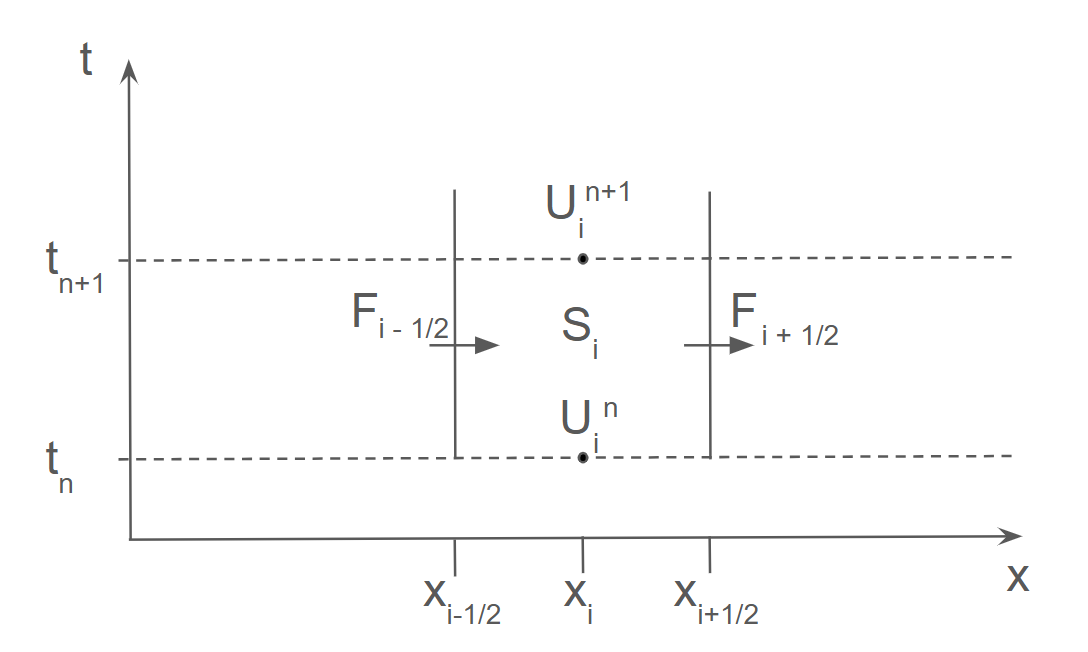
\includegraphics[width=0.5\textwidth]{C:/Users/Matteo/Shallow-Water-Equations/tex/figs/fvm_grid_new.png}
    \caption{Illustration of the grid for the 1D SWE.}\label{fig:10_3}
\end{figure}
The FVM involves discretizing the domain into finite control volumes or cells.
At each cell interface, the local Riemann problem is solved to compute the fluxes, which are then used to update the solution in each cell.
This approach allows for discountinuous solutions, as the Riemann problem is solved at the cell interfaces.
Thus, the FVM is particularly well suited for hyperbolic conservation laws, such as the shallow water equations.

In the context of the 1D Shallow Water Equations (SWE), the FVM is applied by dividing the spatial domain into a set of intervals or grid cells.
Figure~\ref{fig:FVM_1D_grid} illustrates the grid structure used,
\begin{figure}[H]
    \centering
    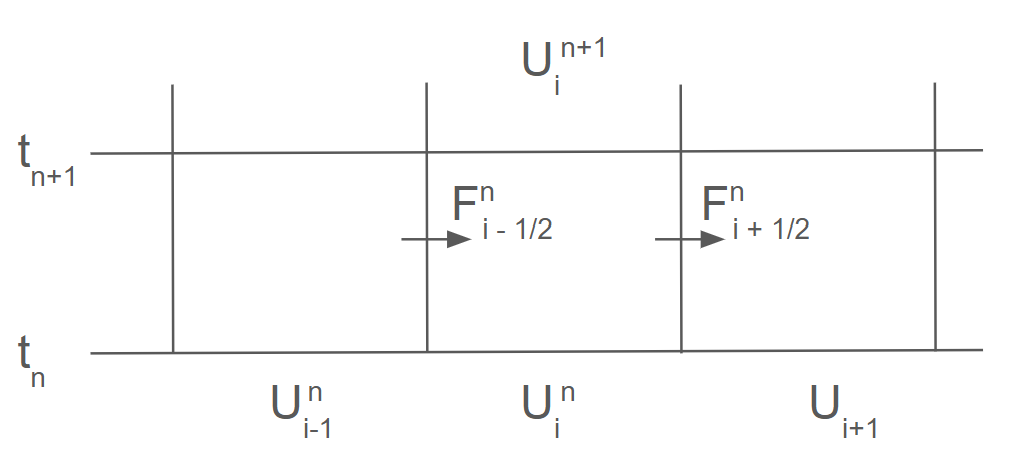
\includegraphics[width=0.5\textwidth]{C:/Users/Matteo/Shallow-Water-Equations/figs/FVM_1D_grid.png}
    \caption{Illustration of the grid for the 1D SWE.}\label{fig:FVM_1D_grid}
\end{figure}

This method, represented by the formula~\eqref{eq:explicit_conservative_1D_SWE}, is referred to as a finite volume scheme, since it is based on the integral conservation over finite volumes.

Finite volume methods are closely related to finite difference methods, but they differs as they are based on the integral form of the conservation laws.
Where finite difference methods tend to break down near discontinuities in the solution, finite volume methods are more suited, since they are based on the integral form of the conservation laws.
The key distinction between the FVM and the Finite Difference Method (FDM) lies in their formulation: while the FVM is based on the integral conservation over finite volumes, the FDM is based on the differential conservation over finite differences.

The central idea of the FVM is to define the numerical flux $\mathbf{F}_{i+1/2}^n$, at the cell interface, as a function of the cell averages $\mathbf{U}_i^n$ and $\mathbf{U}_{i+1}^n$, since the solution is known only in terms of these cell averages.
Consequently, the FVM does not provide pointwise values of the solution, i.e., $\mathbf{U}(x,t)$, but instead gives cell-averaged values, $\mathbf{U}_i^n$, over the control volume.
One of the main challenges in the FVM is to determine appropiate numerical flux functions that, based on the available cell averages, can reasonably approximate the fluxes at the cell interfaces. 



\subsection{Finite Volume Method for the 2D SWE}
Follows the methods outlined in~\cite{Toro2009-Riemann}.
Consider a time-dependent two dimensional system of conservation laws
\begin{align}\label{eq:2D_SWE}
    \mathbf{U}_t + \mathbf{F(U)}_x + \mathbf{G(U)}_y = 0.
\end{align}
A numerical explicit finite volume scheme to solve~\eqref{eq:2D_SWE} is given by
\begin{align}
    \mathbf{U}_{i,j}^{n+1} = \mathbf{U}_{i,j}^n + \frac{\Delta t}{\Delta x}(\mathbf{F}_{i-1/2,j} - \mathbf{F}_{i+1/2,j}) + \frac{\Delta t}{\Delta y}(\mathbf{G}_{i,j-1/2} - \mathbf{G}_{i,j+1/2}).
\end{align}
This is the unsplit finite volume method, meaning that, in a single step, the cell average $\mathbf{U}_{i,j}^n$ is updated using the fluxes from all intercell boundaries.


